\chapter{Análisis del problema}
En este capítulo vamos a realizar un análisis de las funcionalidades que debe cumplir
nuestra aplicación. Para ello, vamos a definir los requisitos funcionales,
no funcionales y de información que debe cumplir. Además, vamos a definir los
casos de uso que se van a dar en nuestra aplicación con sus respectivos diagramas.

\section{Requisitos}
Los actores que van a interactuar con nuestra aplicación son los siguientes:

\begin{itemize}
    \item \textbf{Usuario:} Usuario no registrado en la aplicación. Tendrá funcionalidades
    básicas.
    \item \textbf{Usuario registrado:} Usuario registrado en la aplicación. Tendrá
    acceso a más funcionalidades que el usuario no registrado.
    \item \textbf{Artista:} Usuario registrado con rol de artista. Podrá subir sus
    obras a la aplicación.
    \item \textbf{Administrador:} Usuario registrado con rol de administrador. Podrá
    realizar tareas de administración.
\end{itemize}

\subsection{Requisitos funcionales}
A continuación se van a definir los requisitos funcionales que debe cumplir nuestra
aplicación.

\begin{itemize}
    \item \textbf{RF-1:} Registrarse en la aplicación
    \begin{itemize}
        \item \textbf{RF-1.1:} Registrarse como usuario
        \item \textbf{RF-1.2:} Registrarse como artista
    \end{itemize}
    \item \textbf{RF-2:} Iniciar sesión
    \item \textbf{RF-3:} Eliminar usuario
    \begin{itemize}
        \item \textbf{RF-3.1:} Borrar cuenta como usuario registrado
        \item \textbf{RF-3.2:} Borrar cuenta como administrador
    \end{itemize}
    \item \textbf{RF-4:} Mostrar galería
    \item \textbf{RF-5:} Subir obra en galería
    \item \textbf{RF-6:} Mostrar detalles de obra
    \item \textbf{RF-7:} Valorar obra
    \item \textbf{RF-8:} Mostrar valoraciones de obra
    \item \textbf{RF-9:} Ordenar obras por fecha
    \begin{itemize}
        \item \textbf{RF-9.1:} Ordenar obras fecha descendente
        \item \textbf{RF-9.2:} Ordenar obras fecha ascendente
    \end{itemize}
    \item \textbf{RF-10:} Ordenar obras por valoración
    \begin{itemize}
        \item \textbf{RF-10.1:} Ordenar obras valoración descendente
        \item \textbf{RF-10.2:} Ordenar obras valoración ascendente
    \end{itemize}
    \item \textbf{RF-11:} Filtrar obras por autor
    \item \textbf{RF-12:} Eliminar obra
    \begin{itemize}
        \item \textbf{RF-12.1:} Eliminar obra como artista
        \item \textbf{RF-12.2:} Eliminar obra como administrador
    \end{itemize}
    \item \textbf{RF-13:} Eliminar valoración
    \begin{itemize}
        \item \textbf{RF-13.1:} Eliminar valoración como usuario registrado
        \item \textbf{RF-13.2:} Eliminar valoración como administrador
    \end{itemize}
    \item \textbf{RF-14:} Cerrar sesión
\end{itemize}

\subsection{Requisitos no funcionales}
En cuanto a los requisitos no funcionales, se van a definir los siguientes:

\begin{itemize}
    \item \textbf{RNF-1:} Eficiencia
    \begin{itemize}
        \item \textbf{RNF-1.1:} Toda funcionalidad ha de responder al usuario en menos
        de 5 segundos.
        \item \textbf{RNF-1.2:} La aplicación ha de operar correctamente con hasta 100
        sesiones concurrentes.
        \item \textbf{RNF-1.3:} Los datos modificados en la base de datos tienen que
        estar actualizados en menos de 5 segundos.
    \end{itemize}
    \item \textbf{RNF-2:} Seguridad lógica y de datos
    \begin{itemize}
        \item \textbf{RNF-2.1:} Los permisos de usuario administarador solo pueden ser
        modificados por otro usuario administrador.
        \item \textbf{RNF-2.2:} La aplicación se desarrollará aplicando patrones de
        programación que aumenten la seguirdad de los datos.
        \item \textbf{RNF-2.3:} Los datos sensibles de los usuarios serán encriptados
        antes de almacenarse en la base de datos.
    \end{itemize}
    \item \textbf{RNF-3:} Usabilidad
    \begin{itemize}
        \item \textbf{RNF-3.1:} La aplicación ha de ser intuitiva y fácil de usar por
        personas que no posean grandes conocimientos informáticos.
        \item \textbf{RNF-3.2:} La aplicación cumplirá con los estándares mínimos de
        accesibilidad.
        \item \textbf{RNF-3.3:} Los mensajes de error que proporcione la aplicación
        han de ser informativos y orientados al usuario final.
        \item \textbf{RNF-3.4:} La aplicación ha de ser compatible con los navegadores
        más utilizados.
        \item \textbf{RNF-3.5:} La aplicación ha de tener un diseño responsive, adaptándose
        a diversos tamaños de pantalla y dispositivos.
        \item \textbf{RNF-3.6:} Las imágenes se almacenarán en formato \textit{JPEG} o
        \textit{PNG}.
    \end{itemize}
\end{itemize}

\subsection{Requisitos de información}
Ahora se van a definir los requisitos de información que debe cumplir nuestra
aplicación.

\begin{itemize}
    \item \textbf{RI-1:} Usuario
    \begin{itemize}
        \item \textbf{RI-1.1:} Nombre
        \item \textbf{RI-1.2:} Apellidos
        \item \textbf{RI-1.3:} Correo electrónico
        \item \textbf{RI-1.4:} Contraseña
        \item \textbf{RI-1.5:} Es o no artista
        \item \textbf{RI-1.6:} Es o no administrador
    \end{itemize}
    \item \textbf{RI-2:} Obra
    \begin{itemize}
        \item \textbf{RI-2.1:} Título
        \item \textbf{RI-2.2:} Descripción
        \item \textbf{RI-2.3:} Tipo de obra
        \item \textbf{RI-2.4:} Fecha de creación
        \item \textbf{RI-2.5:} Valoración media
        \item \textbf{RI-2.6:} Autor
        \item \textbf{RI-2.7:} Archivo
    \end{itemize}
    \item \textbf{RI-3:} Valoración
    \begin{itemize}
        \item \textbf{RI-3.1:} Valoración
        \item \textbf{RI-3.2:} Comentario
    \end{itemize}
\end{itemize}

\subsection{Descripción de los requisitos}
A continuación se van a realizar las tablas de descripción de los requisitos funcionales.

\begin{table}[H]
    \centering
    \begin{tabular}{|p{3cm}|p{8cm}|}
        \hline
        \rowcolor{lightgray}
        \textbf{Detalle} & \textbf{Descripción} \\
        \hline
        \textbf{RF\#} & 1.1 \\
        \hline
        \textbf{Nombre} & Registrarse como usuario registrado \\
        \hline
        \textbf{Descripción} & Un usuario podrá registrarse en la aplicación \\
        \hline
        \textbf{Entrada} &
        Agente externo: Usuario
        
        Requisito de datos de entrada: RDE-1.1 \\
        \hline
        \textbf{BD} &
        Requisito de datos de lectura: ninguno
        
        Requisito de datos de escritura: RDW-1.1 \\
        \hline
        \textbf{Salida} & Requisito de datos de salida: ninguno \\
        \hline
        \textbf{RDE-1.1} & Datos de entrada para el registro de un usuario:
            \begin{itemize}
                \item Datos de usuario RI-1
            \end{itemize} \\
        \hline
        \textbf{RDW-1.1} & Datos almacenados de un usuario:
            \begin{itemize}
                \item Datos de usuario RI-1
            \end{itemize} \\
        \hline
    \end{tabular}
    \caption{Descripción del requisito funcional RF-1.1}
    \label{tab:rf-1-1}
\end{table}

\begin{table}[H]
    \centering
    \begin{tabular}{|p{3cm}|p{8cm}|}
        \hline
        \rowcolor{lightgray}
        \textbf{Detalle} & \textbf{Descripción} \\
        \hline
        \textbf{RF\#} & 1.2 \\
        \hline
        \textbf{Nombre} & Registrarse como artista \\
        \hline
        \textbf{Descripción} & Un usuario podrá registrarse en la aplicación como artista \\
        \hline
        \textbf{Entrada} &
        Agente externo: Usuario
        
        Requisito de datos de entrada: RDE-1.2 \\
        \hline
        \textbf{BD} &
        Requisito de datos de lectura: ninguno
        
        Requisito de datos de escritura: RDW-1.2 \\
        \hline
        \textbf{Salida} & Requisito de datos de salida: ninguno \\
        \hline
        \textbf{RDE-1.2} & Datos de entrada para el registro de un usuario como artista:
            \begin{itemize}
                \item Usuario RI-1
            \end{itemize} \\
        \hline
        \textbf{RDW-1.2} & Datos almacenados de un usuario:
            \begin{itemize}
                \item Usuario RI-1
            \end{itemize} \\
        \hline
    \end{tabular}
    \caption{Descripción del requisito funcional RF-1.2}
    \label{tab:rf-1-2}
\end{table}

\begin{table}[H]
    \centering
    \begin{tabular}{|p{3cm}|p{8cm}|}
        \hline
        \rowcolor{lightgray}
        \textbf{Detalle} & \textbf{Descripción} \\
        \hline
        \textbf{RF\#} & 2 \\
        \hline
        \textbf{Nombre} & Iniciar sesión \\
        \hline
        \textbf{Descripción} & Un usuario podrá iniciar sesión en la aplicación \\
        \hline
        \textbf{Entrada} &
        Agente externo: Usuario
        
        Requisito de datos de entrada: RDE-2 \\
        \hline
        \textbf{BD} &
        Requisito de datos de lectura: RDR-2
        
        Requisito de datos de escritura: ninguno \\
        \hline
        \textbf{Salida} & Requisito de datos de salida: ninguno \\
        \hline
        \textbf{RDE-2} & Datos de entrada para iniciar sesión:
            \begin{itemize}
                \item Correo electrónico RI-1.3
                \item Contraseña RI-1.4
            \end{itemize} \\
        \hline
        \textbf{RDR-2} & Datos de lectura de un usuario:
            \begin{itemize}
                \item Usuario RI-1
            \end{itemize} \\
        \hline
    \end{tabular}
    \caption{Descripción del requisito funcional RF-2}
    \label{tab:rf-2}
\end{table}

\begin{table}[H]
    \centering
    \begin{tabular}{|p{3cm}|p{8cm}|}
        \hline
        \rowcolor{lightgray}
        \textbf{Detalle} & \textbf{Descripción} \\
        \hline
        \textbf{RF\#} & 3.1 \\
        \hline
        \textbf{Nombre} & Borrar cuenta como usuario registrado \\
        \hline
        \textbf{Descripción} & Un usuario registrado podrá borrar su cuenta \\
        \hline
        \textbf{Entrada} &
        Agente externo: Usuario registrado
        
        Requisito de datos de entrada: ninguno \\
        \hline
        \textbf{BD} &
        Requisito de datos de lectura: RDR-3.1
        
        Requisito de datos de escritura: RDW-3.1 \\
        \hline
        \textbf{Salida} & Requisito de datos de salida: ninguno \\
        \hline
        \textbf{RDR-3.1} & Datos de lectura para borrar un usuario:
            \begin{itemize}
                \item Usuario RI-1
                \item Obras del usuario RI-2
            \end{itemize} \\
        \hline
        \textbf{RDW-3.1} & Datos de escritura de un usuario:
            \begin{itemize}
                \item Eliminar usuario RI-1
                \item Eliminar obras del usuario RI-2
            \end{itemize} \\
        \hline
    \end{tabular}
    \caption{Descripción del requisito funcional RF-3.1}
    \label{tab:rf-3-1}
\end{table}

\begin{table}[H]
    \centering
    \begin{tabular}{|p{3cm}|p{8cm}|}
        \hline
        \rowcolor{lightgray}
        \textbf{Detalle} & \textbf{Descripción} \\
        \hline
        \textbf{RF\#} & 3.2 \\
        \hline
        \textbf{Nombre} & Borrar cuenta como administrador \\
        \hline
        \textbf{Descripción} & Un administrador podrá borrar la cuenta de un usuario \\
        \hline
        \textbf{Entrada} &
        Agente externo: Administrador
        
        Requisito de datos de entrada: RDE-3.2 \\
        \hline
        \textbf{BD} &
        Requisito de datos de lectura: RDR-3.2
        
        Requisito de datos de escritura: RDW-3.2 \\
        \hline
        \textbf{Salida} & Requisito de datos de salida: ninguno \\
        \hline
        \textbf{RDE-3.2} & Datos de entrada para borrar un usuario:
            \begin{itemize}
                \item Usuario RI-1
            \end{itemize} \\
        \hline
        \textbf{RDR-3.2} & Datos de lectura para borrar un usuario:
            \begin{itemize}
                \item Usuario RI-1
                \item Obras del usuario RI-2
            \end{itemize} \\
        \hline
        \textbf{RDW-3.2} & Datos de escritura para borrar un usuario:
            \begin{itemize}
                \item Eliminar usuario RI-1
                \item Eliminar obras del usuario RI-2
            \end{itemize} \\
        \hline
    \end{tabular}
    \caption{Descripción del requisito funcional RF-3.2}
    \label{tab:rf-3-2}
\end{table}

\begin{table}[H]
    \centering
    \begin{tabular}{|p{3cm}|p{8cm}|}
        \hline
        \rowcolor{lightgray}
        \textbf{Detalle} & \textbf{Descripción} \\
        \hline
        \textbf{RF\#} & 4 \\
        \hline
        \textbf{Nombre} & Mostrar galería \\
        \hline
        \textbf{Descripción} & Mostrar todas las obras de la galería \\
        \hline
        \textbf{Entrada} &
        Agente externo: Usuario
        
        Requisito de datos de entrada: RDE-4 \\
        \hline
        \textbf{BD} &
        Requisito de datos de lectura: RDR-4
        
        Requisito de datos de escritura: ninguno \\
        \hline
        \textbf{Salida} & Requisito de datos de salida: RDS-4 \\
        \hline
        \textbf{RDE-4} & Datos de entrada para mostrar la galería:
            \begin{itemize}
                \item Tipo de obra RI-2.3
            \end{itemize} \\
        \hline
        \textbf{RDR-4} & Datos de lectura para mostrar la galería:
            \begin{itemize}
                \item Obras RI-2
            \end{itemize} \\
        \hline
        \textbf{RDS-4} & Datos de salida para mostrar la galería:
            \begin{itemize}
                \item Obras RI-2
            \end{itemize} \\
        \hline
    \end{tabular}
    \caption{Descripción del requisito funcional RF-4}
    \label{tab:rf-4}
\end{table}

\begin{table}[H]
    \centering
    \begin{tabular}{|p{3cm}|p{8cm}|}
        \hline
        \rowcolor{lightgray}
        \textbf{Detalle} & \textbf{Descripción} \\
        \hline
        \textbf{RF\#} & 5 \\
        \hline
        \textbf{Nombre} & Subir obra en galería \\
        \hline
        \textbf{Descripción} & Un artista podrá subir una obra a la galería \\
        \hline
        \textbf{Entrada} &
        Agente externo: Artista
        
        Requisito de datos de entrada: RDE-5 \\
        \hline
        \textbf{BD} &
        Requisito de datos de lectura: ninguno
        
        Requisito de datos de escritura: RDW-5 \\
        \hline
        \textbf{Salida} & Requisito de datos de salida: ninguno \\
        \hline
        \textbf{RDE-5} & Datos de entrada para subir una obra:
            \begin{itemize}
                \item Obra RI-2
            \end{itemize} \\
        \hline
        \textbf{RDW-5} & Datos de escritura para subir una obra:
            \begin{itemize}
                \item Obra RI-2
            \end{itemize} \\
        \hline
    \end{tabular}
    \caption{Descripción del requisito funcional RF-5}
    \label{tab:rf-5}
\end{table}

\begin{table}[H]
    \centering
    \begin{tabular}{|p{3cm}|p{8cm}|}
        \hline
        \rowcolor{lightgray}
        \textbf{Detalle} & \textbf{Descripción} \\
        \hline
        \textbf{RF\#} & 6 \\
        \hline
        \textbf{Nombre} & Mostrar detalles de obra \\
        \hline
        \textbf{Descripción} & Mostrar los detalles de una obra \\
        \hline
        \textbf{Entrada} &
        Agente externo: Usuario
        
        Requisito de datos de entrada: RDE-6 \\
        \hline
        \textbf{BD} &
        Requisito de datos de lectura: RDR-6
        
        Requisito de datos de escritura: ninguno \\
        \hline
        \textbf{Salida} & Requisito de datos de salida: RDS-6 \\
        \hline
        \textbf{RDE-6} & Datos de entrada para mostrar los detalles de una obra:
            \begin{itemize}
                \item Obra RI-2
            \end{itemize} \\
        \hline
        \textbf{RDR-6} & Datos de lectura para mostrar los detalles de una obra:
            \begin{itemize}
                \item Contenido obra RI-2.7
            \end{itemize} \\
        \hline
        \textbf{RDS-6} & Datos de salida para mostrar los detalles de una obra:
            \begin{itemize}
                \item Contenido obra RI-2.7
            \end{itemize} \\
        \hline
    \end{tabular}
    \caption{Descripción del requisito funcional RF-6}
    \label{tab:rf-6}
\end{table}

\begin{table}[H]
    \centering
    \begin{tabular}{|p{3cm}|p{8cm}|}
        \hline
        \rowcolor{lightgray}
        \textbf{Detalle} & \textbf{Descripción} \\
        \hline
        \textbf{RF\#} & 7 \\
        \hline
        \textbf{Nombre} & Valorar obra \\
        \hline
        \textbf{Descripción} & Un usuario registrado podrá valorar una obra con
        una puntuación y un comentario opcionalmente \\
        \hline
        \textbf{Entrada} &
        Agente externo: Usuario registrado
        
        Requisito de datos de entrada: RDE-7 \\
        \hline
        \textbf{BD} &
        Requisito de datos de lectura: ninguno
        
        Requisito de datos de escritura: RDW-7 \\
        \hline
        \textbf{Salida} & Requisito de datos de salida: ninguno \\
        \hline
        \textbf{RDE-7} & Datos de entrada para valorar una obra:
            \begin{itemize}
                \item Obra RI-2
                \item Valoración RI-3.1
                \item Comentario RI-3.2
            \end{itemize} \\
        \hline
        \textbf{RDW-7} & Datos de escritura para valorar una obra:
            \begin{itemize}
                \item Valoración RI-3
            \end{itemize} \\
        \hline
    \end{tabular}
    \caption{Descripción del requisito funcional RF-7}
    \label{tab:rf-7}
\end{table}

\begin{table}[H]
    \centering
    \begin{tabular}{|p{3cm}|p{8cm}|}
        \hline
        \rowcolor{lightgray}
        \textbf{Detalle} & \textbf{Descripción} \\
        \hline
        \textbf{RF\#} & 8 \\
        \hline
        \textbf{Nombre} & Mostrar valoraciones de obra \\
        \hline
        \textbf{Descripción} & Mostrar las valoraciones de una obra \\
        \hline
        \textbf{Entrada} &
        Agente externo: Usuario
        
        Requisito de datos de entrada: RDE-8 \\
        \hline
        \textbf{BD} &
        Requisito de datos de lectura: RDR-8
        
        Requisito de datos de escritura: ninguno \\
        \hline
        \textbf{Salida} & Requisito de datos de salida: RDS-8 \\
        \hline
        \textbf{RDE-8} & Datos de entrada para mostrar las valoraciones de una obra:
            \begin{itemize}
                \item Obra RI-2
            \end{itemize} \\
        \hline
        \textbf{RDR-8} & Datos de lectura para mostrar las valoraciones de una obra:
            \begin{itemize}
                \item Valoraciones RI-3
            \end{itemize} \\
        \hline
        \textbf{RDS-8} & Datos de salida para mostrar las valoraciones de una obra:
            \begin{itemize}
                \item Valoraciones RI-3
            \end{itemize} \\
        \hline
    \end{tabular}
    \caption{Descripción del requisito funcional RF-8}
    \label{tab:rf-8}
\end{table}

\begin{table}[H]
    \centering
    \begin{tabular}{|p{3cm}|p{8cm}|}
        \hline
        \rowcolor{lightgray}
        \textbf{Detalle} & \textbf{Descripción} \\
        \hline
        \textbf{RF\#} & 9.1 \\
        \hline
        \textbf{Nombre} & Ordenar obras por fecha descendente \\
        \hline
        \textbf{Descripción} & Un usuario podrá visualizar las obras ordenadas
        por fecha de creación de forma descendente \\
        \hline
        \textbf{Entrada} &
        Agente externo: Usuario
        
        Requisito de datos de entrada: ninguno \\
        \hline
        \textbf{BD} &
        Requisito de datos de lectura: RDR-9.1
        
        Requisito de datos de escritura: ninguno \\
        \hline
        \textbf{Salida} & Requisito de datos de salida: RDS-9.1 \\
        \hline
        \textbf{RDR-9.1} & Datos de lectura para mostrar las obras ordenadas por fecha
        de creación de forma descendente:
            \begin{itemize}
                \item Obras RI-2
                \item Fecha de creación RI-2.4
            \end{itemize} \\
        \hline
        \textbf{RDS-9.1} & Datos de salida para mostrar las obras ordenadas por fecha
        de creación de forma descendente:
            \begin{itemize}
                \item Obras RI-2
            \end{itemize} \\
        \hline
    \end{tabular}
    \caption{Descripción del requisito funcional RF-9.1}
    \label{tab:rf-9-1}
\end{table}

\begin{table}[H]
    \centering
    \begin{tabular}{|p{3cm}|p{8cm}|}
        \hline
        \rowcolor{lightgray}
        \textbf{Detalle} & \textbf{Descripción} \\
        \hline
        \textbf{RF\#} & 9.2 \\
        \hline
        \textbf{Nombre} & Ordenar obras por fecha ascendente \\
        \hline
        \textbf{Descripción} & Un usuario podrá visualizar las obras ordenadas
        por fecha de creación de forma ascendente \\
        \hline
        \textbf{Entrada} &
        Agente externo: Usuario
        
        Requisito de datos de entrada: ninguno \\
        \hline
        \textbf{BD} &
        Requisito de datos de lectura: RDR-9.2
        
        Requisito de datos de escritura: ninguno \\
        \hline
        \textbf{Salida} & Requisito de datos de salida: RDS-9.2 \\
        \hline
        \textbf{RDR-9.2} & Datos de lectura para mostrar las obras ordenadas por fecha
        de creación de forma ascendente:
            \begin{itemize}
                \item Obras RI-2
                \item Fecha de creación RI-2.4
            \end{itemize} \\
        \hline
        \textbf{RDS-9.2} & Datos de salida para mostrar las obras ordenadas por fecha
        de creación de forma ascendente:
            \begin{itemize}
                \item Obras RI-2
            \end{itemize} \\
        \hline
    \end{tabular}
    \caption{Descripción del requisito funcional RF-9.2}
    \label{tab:rf-9-2}
\end{table}

\begin{table}[H]
    \centering
    \begin{tabular}{|p{3cm}|p{8cm}|}
        \hline
        \rowcolor{lightgray}
        \textbf{Detalle} & \textbf{Descripción} \\
        \hline
        \textbf{RF\#} & 10.1 \\
        \hline
        \textbf{Nombre} & Ordenar obras por valoración descendente \\
        \hline
        \textbf{Descripción} & Un usuario podrá visualizar las obras ordenadas
        por valoración de forma descendente \\
        \hline
        \textbf{Entrada} &
        Agente externo: Usuario
        
        Requisito de datos de entrada: ninguno \\
        \hline
        \textbf{BD} &
        Requisito de datos de lectura: RDR-10.1
        
        Requisito de datos de escritura: ninguno \\
        \hline
        \textbf{Salida} & Requisito de datos de salida: RDS-10.1 \\
        \hline
        \textbf{RDR-10.1} & Datos de lectura para mostrar las obras ordenadas por valoración
        de forma descendente:
            \begin{itemize}
                \item Obras RI-2
                \item Valoración media RI-2.5
            \end{itemize} \\
        \hline
        \textbf{RDS-10.1} & Datos de salida para mostrar las obras ordenadas por valoración
        de forma descendente:
            \begin{itemize}
                \item Obras RI-2
            \end{itemize} \\
        \hline
    \end{tabular}
    \caption{Descripción del requisito funcional RF-10.1}
    \label{tab:rf-10-1}
\end{table}

\begin{table}[H]
    \centering
    \begin{tabular}{|p{3cm}|p{8cm}|}
        \hline
        \rowcolor{lightgray}
        \textbf{Detalle} & \textbf{Descripción} \\
        \hline
        \textbf{RF\#} & 10.2 \\
        \hline
        \textbf{Nombre} & Ordenar obras por valoración ascendente \\
        \hline
        \textbf{Descripción} & Un usuario podrá visualizar las obras ordenadas
        por valoración de forma ascendente \\
        \hline
        \textbf{Entrada} &
        Agente externo: Usuario
        
        Requisito de datos de entrada: ninguno \\
        \hline
        \textbf{BD} &
        Requisito de datos de lectura: RDR-10.2
        
        Requisito de datos de escritura: ninguno \\
        \hline
        \textbf{Salida} & Requisito de datos de salida: RDS-10.2 \\
        \hline
        \textbf{RDR-10.2} & Datos de lectura para mostrar las obras ordenadas por valoración
        de forma ascendente:
            \begin{itemize}
                \item Obras RI-2
                \item Valoración media RI-2.5
            \end{itemize} \\
        \hline
        \textbf{RDS-10.2} & Datos de salida para mostrar las obras ordenadas por valoración
        de forma ascendente:
            \begin{itemize}
                \item Obras RI-2
            \end{itemize} \\
        \hline
    \end{tabular}
    \caption{Descripción del requisito funcional RF-10.2}
    \label{tab:rf-10-2}
\end{table}

\begin{table}[H]
    \centering
    \begin{tabular}{|p{3cm}|p{8cm}|}
        \hline
        \rowcolor{lightgray}
        \textbf{Detalle} & \textbf{Descripción} \\
        \hline
        \textbf{RF\#} & 11 \\
        \hline
        \textbf{Nombre} & Filtrar obras por autor \\
        \hline
        \textbf{Descripción} & Un usuario podrá visualizar las obras de un autor
        concreto \\
        \hline
        \textbf{Entrada} &
        Agente externo: Usuario
        
        Requisito de datos de entrada: RDE-11 \\
        \hline
        \textbf{BD} &
        Requisito de datos de lectura: RDR-11
        
        Requisito de datos de escritura: ninguno \\
        \hline
        \textbf{Salida} & Requisito de datos de salida: RDS-11 \\
        \hline
        \textbf{RDE-11} & Datos de entrada para mostrar las obras de un autor:
            \begin{itemize}
                \item Autor RI-2.6
            \end{itemize} \\
        \hline
        \textbf{RDR-11} & Datos de lectura para mostrar las obras de un autor:
            \begin{itemize}
                \item Obras RI-2
                \item Autor RI-2.6
            \end{itemize} \\
        \hline
        \textbf{RDS-11} & Datos de salida para mostrar las obras de un autor:
            \begin{itemize}
                \item Obras RI-2
            \end{itemize} \\
        \hline
    \end{tabular}
    \caption{Descripción del requisito funcional RF-11}
    \label{tab:rf-11}
\end{table}

\begin{table}[H]
    \centering
    \begin{tabular}{|p{3cm}|p{8cm}|}
        \hline
        \rowcolor{lightgray}
        \textbf{Detalle} & \textbf{Descripción} \\
        \hline
        \textbf{RF\#} & 12.1 \\
        \hline
        \textbf{Nombre} & Eliminar obra como artista \\
        \hline
        \textbf{Descripción} & Un artista podrá eliminar una obra suya \\
        \hline
        \textbf{Entrada} &
        Agente externo: Artista

        Requisito de datos de entrada: RDE-12.1 \\
        \hline
        \textbf{BD} &
        Requisito de datos de lectura: RDR-12.1

        Requisito de datos de escritura: RDW-12.1 \\
        \hline
        \textbf{Salida} & Requisito de datos de salida: ninguno \\
        \hline
        \textbf{RDE-12.1} & Datos de entrada para eliminar una obra:
            \begin{itemize}
                \item Obra RI-2
            \end{itemize} \\
        \hline
        \textbf{RDR-12.1} & Datos de lectura para eliminar una obra:
            \begin{itemize}
                \item Obra RI-2
            \end{itemize} \\
        \hline
        \textbf{RDW-12.1} & Datos de escritura para eliminar una obra:
            \begin{itemize}
                \item Eliminar obra RI-2
            \end{itemize} \\
        \hline
    \end{tabular}
    \caption{Descripción del requisito funcional RF-12.1}
    \label{tab:rf-12-1}
\end{table}

\begin{table}[H]
    \centering
    \begin{tabular}{|p{3cm}|p{8cm}|}
        \hline
        \rowcolor{lightgray}
        \textbf{Detalle} & \textbf{Descripción} \\
        \hline
        \textbf{RF\#} & 12.2 \\
        \hline
        \textbf{Nombre} & Eliminar obra como administrador \\
        \hline
        \textbf{Descripción} & Un administrador podrá eliminar una obra de un artista \\
        \hline
        \textbf{Entrada} &
        Agente externo: Administrador

        Requisito de datos de entrada: RDE-12.2 \\
        \hline
        \textbf{BD} &
        Requisito de datos de lectura: RDR-12.2

        Requisito de datos de escritura: RDW-12.2 \\
        \hline
        \textbf{Salida} & Requisito de datos de salida: ninguno \\
        \hline
        \textbf{RDE-12.2} & Datos de entrada para eliminar una obra:
            \begin{itemize}
                \item Obra RI-2
            \end{itemize} \\
        \hline
        \textbf{RDR-12.2} & Datos de lectura para eliminar una obra:
            \begin{itemize}
                \item Obra RI-2
            \end{itemize} \\
        \hline
        \textbf{RDW-12.2} & Datos de escritura para eliminar una obra:
            \begin{itemize}
                \item Eliminar obra RI-2
            \end{itemize} \\
        \hline
    \end{tabular}
    \caption{Descripción del requisito funcional RF-12.2}
    \label{tab:rf-12-2}
\end{table}

\begin{table}[H]
    \centering
    \begin{tabular}{|p{3cm}|p{8cm}|}
        \hline
        \rowcolor{lightgray}
        \textbf{Detalle} & \textbf{Descripción} \\
        \hline
        \textbf{RF\#} & 13.1 \\
        \hline
        \textbf{Nombre} & Eliminar valoración como usuario registrado \\
        \hline
        \textbf{Descripción} & Un usuario registrado podrá eliminar una valoración suya \\
        \hline
        \textbf{Entrada} &
        Agente externo: Usuario registrado

        Requisito de datos de entrada: RDE-13.1 \\
        \hline
        \textbf{BD} &
        Requisito de datos de lectura: RDR-13.1

        Requisito de datos de escritura: RDW-13.1 \\
        \hline
        \textbf{Salida} & Requisito de datos de salida: ninguno \\
        \hline
        \textbf{RDE-13.1} & Datos de entrada para eliminar una valoración:
            \begin{itemize}
                \item Valoración RI-3
            \end{itemize} \\
        \hline
        \textbf{RDR-13.1} & Datos de lectura para eliminar una valoración:
            \begin{itemize}
                \item Valoración RI-3
            \end{itemize} \\
        \hline
        \textbf{RDW-13.1} & Datos de escritura para eliminar una valoración:
            \begin{itemize}
                \item Eliminar valoración RI-3
            \end{itemize} \\
        \hline
    \end{tabular}
    \caption{Descripción del requisito funcional RF-13.1}
    \label{tab:rf-13-1}
\end{table}

\begin{table}[H]
    \centering
    \begin{tabular}{|p{3cm}|p{8cm}|}
        \hline
        \rowcolor{lightgray}
        \textbf{Detalle} & \textbf{Descripción} \\
        \hline
        \textbf{RF\#} & 13.2 \\
        \hline
        \textbf{Nombre} & Eliminar valoración como administrador \\
        \hline
        \textbf{Descripción} & Un administrador podrá eliminar una valoración de un usuario \\
        \hline
        \textbf{Entrada} &
        Agente externo: Administrador

        Requisito de datos de entrada: RDE-13.2 \\
        \hline
        \textbf{BD} &
        Requisito de datos de lectura: RDR-13.2

        Requisito de datos de escritura: RDW-13.2 \\
        \hline
        \textbf{Salida} & Requisito de datos de salida: ninguno \\
        \hline
        \textbf{RDE-13.2} & Datos de entrada para eliminar una valoración:
            \begin{itemize}
                \item Valoración RI-3
            \end{itemize} \\
        \hline
        \textbf{RDR-13.2} & Datos de lectura para eliminar una valoración:
            \begin{itemize}
                \item Valoración RI-3
            \end{itemize} \\
        \hline
        \textbf{RDW-13.2} & Datos de escritura para eliminar una valoración:
            \begin{itemize}
                \item Eliminar valoración RI-3
            \end{itemize} \\
        \hline
    \end{tabular}
    \caption{Descripción del requisito funcional RF-13.2}
    \label{tab:rf-13-2}
\end{table}

\begin{table}[H]
    \centering
    \begin{tabular}{|p{3cm}|p{8cm}|}
        \hline
        \rowcolor{lightgray}
        \rowcolor{lightgray}
        \textbf{Detalle} & \textbf{Descripción} \\
        \hline
        \textbf{RF\#} & 14 \\
        \hline
        \textbf{Nombre} & Cerrar sesión \\
        \hline
        \textbf{Descripción} & Un usuario podrá cerrar sesión en la aplicación \\
        \hline
        \textbf{Entrada} &
        Agente externo: Usuario

        Requisito de datos de entrada: ninguno \\
        \hline
        \textbf{BD} &
        Requisito de datos de lectura: ninguno

        Requisito de datos de escritura: ninguno \\
        \hline
        \textbf{Salida} & Requisito de datos de salida: ninguno \\
        \hline
    \end{tabular}
    \caption{Descripción del requisito funcional RF-14}
    \label{tab:rf-14}
\end{table}

\section{Casos de uso}
En esta sección se van a describir los casos de uso que se pueden dar
en la aplicación. En primer lugar difiniremos los actores que van a realizar
los casos de uso y después se definirán los casos de uso con sus respectivos
diagramas.

\subsection{Actores}
Se van a definir las tablas con las características de los actores y los casos
de uso en los que se referencian:

\begin{table}[H]
    \begin{tabular}{|p{3cm}|p{5cm}|p{2cm}|}
        \hline
        Actor & Usuario & ACT-1 \\
        \hline
        Descripción & \multicolumn{2}{|p{7cm}|}{Usuario no registrado
        que utiliza la aplicación.} \\
        \hline
        Características & \multicolumn{2}{|p{7cm}|}{Puede ser cualquier persona
        que entre en la aplicación.} \\
        \hline
        Relaciones & \multicolumn{2}{|c|}{-} \\
        \hline
        Referencias & \multicolumn{2}{|p{7cm}|}{CU-1, CU-5, CU-7, CU-9, CU-10,
        CU-11} \\
        \hline
    \end{tabular}
    \caption{Definición del actor Usuario}
    \label{tab:actor_usuario}
\end{table}

\begin{table}[H]
    \begin{tabular}{|p{3cm}|p{5cm}|p{2cm}|}
        \hline
        Actor & Usuario registrado & ACT-2 \\
        \hline
        Descripción & \multicolumn{2}{|p{7cm}|}{Usuario registrado en la aplicación.} \\
        \hline
        Características & \multicolumn{2}{|p{7cm}|}{Es cualquier usuario que esté
        registrado y haya iniciado sesión.} \\
        \hline
        Relaciones & \multicolumn{2}{|p{7cm}|}{Es un usuario} \\
        \hline
        Referencias & \multicolumn{2}{|p{7cm}|}{CU-2, CU-3, CU-4, CU-8, CU-14,
        CU-15, CU-16} \\
        \hline
    \end{tabular}
    \caption{Definición del actor Usuario registrado}
    \label{tab:actor_usuario_registrado}
\end{table}

\begin{table}[H]
    \begin{tabular}{|p{3cm}|p{5cm}|p{2cm}|}
        \hline
        Actor & Artista & ACT-3 \\
        \hline
        Descripción & \multicolumn{2}{|p{7cm}|}{Usuario registrado con rol de artista.} \\
        \hline
        Características & \multicolumn{2}{|p{7cm}|}{Es un usuario registrado que
        va a subir obras a alguna galería de la aplicación.} \\
        \hline
        Relaciones & \multicolumn{2}{|p{7cm}|}{Es un usuario registrado} \\
        \hline
        Referencias & \multicolumn{2}{|p{7cm}|}{CU-6, CU-12, CU-13} \\
        \hline
    \end{tabular}
    \caption{Definición del actor Artista}
    \label{tab:actor_artista}
\end{table}

\begin{table}[H]
    \begin{tabular}{|p{3cm}|p{5cm}|p{2cm}|}
        \hline
        Actor & Administrador & ACT-4 \\
        \hline
        Descripción & \multicolumn{2}{|p{7cm}|}{Usuario con permisos especiales para
        administrar la aplicación.} \\
        \hline
        Características & \multicolumn{2}{|p{7cm}|}{Es un usuario que podrá administrar
        el contenido y los usuarios de la aplicación.} \\
        \hline
        Relaciones & \multicolumn{2}{|p{7cm}|}{Es un usuario registrado} \\
        \hline
        Referencias & \multicolumn{2}{|p{7cm}|}{CU-4, CU-13, CU-15} \\
        \hline
    \end{tabular}
    \caption{Definición del actor Administrador}
    \label{tab:actor_administrador}
\end{table}

\subsection{Definición de casos de uso}
A continuación se van a definir los casos de uso de la aplicación especificando
el tipo de los mismos y los actores que intervienen en cada uno de ellos:

\begin{table}[H]
    \begin{tabular}{|p{3cm}|p{5cm}|p{2cm}|}
        \hline
        Caso de uso & Registrarse en la aplicación & CU-1 \\
        \hline
        Actores & \multicolumn{2}{|p{7cm}|}{Usuario (principal)} \\
        \hline
        Tipo & \multicolumn{2}{|p{7cm}|}{Primario y esencial} \\
        \hline
        Referencias & RF-1 & \multicolumn{1}{|c|}{-} \\
        \hline
        Precondición & \multicolumn{2}{|p{7cm}|}{El usuario no está registrado
        en la aplicación} \\
        \hline
        Postcondición & \multicolumn{2}{|p{7cm}|}{El sistema habrá guardado la
        información correspondiente al registro del usuario} \\
        \hline
    \end{tabular}
    \caption{Definición del caso de uso CU-1}
    \label{tab:cu_1}
\end{table}

\begin{table}[H]
    \begin{tabular}{|p{3cm}|p{5cm}|p{2cm}|}
        \hline
        Caso de uso & Iniciar sesión & CU-2 \\
        \hline
        Actores & \multicolumn{2}{|p{7cm}|}{Usuario (principal)} \\
        \hline
        Tipo & \multicolumn{2}{|p{7cm}|}{Primario y esencial} \\
        \hline
        Referencias & RF-2 & \multicolumn{1}{|c|}{-} \\
        \hline
        Precondición & \multicolumn{2}{|p{7cm}|}{El usuario está registrado
        en la aplicación} \\
        \hline
        Postcondición & \multicolumn{2}{|p{7cm}|}{El sistema crea una sesión para
        el usuario y reconoce que es ese usuario concreto el que está utilizando la aplicación} \\
        \hline
    \end{tabular}
    \caption{Definición del caso de uso CU-2}
    \label{tab:cu_2}
\end{table}

\begin{table}[H]
    \begin{tabular}{|p{3cm}|p{5cm}|p{2cm}|}
        \hline
        Caso de uso & Eliminar cuenta como usuario registrado & CU-3 \\
        \hline
        Actores & \multicolumn{2}{|p{7cm}|}{Usuario registrado (principal)} \\
        \hline
        Tipo & \multicolumn{2}{|p{7cm}|}{Primario y esencial} \\
        \hline
        Referencias & RF-3.1 & \multicolumn{1}{|c|}{-} \\
        \hline
        Precondición & \multicolumn{2}{|p{7cm}|}{El usuario está registrado
        en la aplicación} \\
        \hline
        Postcondición & \multicolumn{2}{|p{7cm}|}{El sistema elimina la información
        correspondiente al usuario} \\
        \hline
    \end{tabular}
    \caption{Definición del caso de uso CU-3}
    \label{tab:cu_3}
\end{table}

\begin{table}[H]
    \begin{tabular}{|p{3cm}|p{5cm}|p{2cm}|}
        \hline
        Caso de uso & Eliminar cuenta como administrador & CU-4 \\
        \hline
        Actores & \multicolumn{2}{|p{7cm}|}{Administrador (principal)
        y Usuario registrado (secundario)} \\
        \hline
        Tipo & \multicolumn{2}{|p{7cm}|}{Primario y esencial} \\
        \hline
        Referencias & RF-3.2 & \multicolumn{1}{|c|}{-} \\
        \hline
        Precondición & \multicolumn{2}{|p{7cm}|}{El usuario está registrado
        en la aplicación} \\
        \hline
        Postcondición & \multicolumn{2}{|p{7cm}|}{El sistema elimina la información
        correspondiente al usuario} \\
        \hline
    \end{tabular}
    \caption{Definición del caso de uso CU-4}
    \label{tab:cu_4}
\end{table}

\begin{table}[H]
    \begin{tabular}{|p{3cm}|p{5cm}|p{2cm}|}
        \hline
        Caso de uso & Visitar galería de arte & CU-5 \\
        \hline
        Actores & \multicolumn{2}{|p{7cm}|}{Usuario (principal)} \\
        \hline
        Tipo & \multicolumn{2}{|p{7cm}|}{Primario y esencial} \\
        \hline
        Referencias & RF-4 & \multicolumn{1}{|c|}{-} \\
        \hline
        Precondición & \multicolumn{2}{|p{7cm}|}{Ninguna} \\
        \hline
        Postcondición & \multicolumn{2}{|p{7cm}|}{Se muestra el contenido
        de la galería} \\
        \hline
    \end{tabular}
    \caption{Definición del caso de uso CU-5}
    \label{tab:cu_5}
\end{table}

\begin{table}[H]
    \begin{tabular}{|p{3cm}|p{5cm}|p{2cm}|}
        \hline
        Caso de uso & Subir obra & CU-6 \\
        \hline
        Actores & \multicolumn{2}{|p{7cm}|}{Artista (principal)} \\
        \hline
        Tipo & \multicolumn{2}{|p{7cm}|}{Primario y esencial} \\
        \hline
        Referencias & RF-5 & \multicolumn{1}{|c|}{-} \\
        \hline
        Precondición & \multicolumn{2}{|p{7cm}|}{La obra se encuentra en
        un formato soportado por la galería a la que se va a subir} \\
        \hline
        Postcondición & \multicolumn{2}{|p{7cm}|}{El sistema guarda la información
        correspondiente a la obra} \\
        \hline
    \end{tabular}
    \caption{Definición del caso de uso CU-6}
    \label{tab:cu_6}
\end{table}

\begin{table}[H]
    \begin{tabular}{|p{3cm}|p{5cm}|p{2cm}|}
        \hline
        Caso de uso & Mostrar detalles de obra & CU-7 \\
        \hline
        Actores & \multicolumn{2}{|p{7cm}|}{Usuario (principal)} \\
        \hline
        Tipo & \multicolumn{2}{|p{7cm}|}{Primario y esencial} \\
        \hline
        Referencias & RF-6 & \multicolumn{1}{|c|}{-} \\
        \hline
        Precondición & \multicolumn{2}{|p{7cm}|}{La obra existe en la galería} \\
        \hline
        Postcondición & \multicolumn{2}{|p{7cm}|}{Se muestra la información
        correspondiente a la obra} \\
        \hline
    \end{tabular}
    \caption{Definición del caso de uso CU-7}
    \label{tab:cu_7}
\end{table}

\begin{table}[H]
    \begin{tabular}{|p{3cm}|p{5cm}|p{2cm}|}
        \hline
        Caso de uso & Valorar obra & CU-8 \\
        \hline
        Actores & \multicolumn{2}{|p{7cm}|}{Usuario registrado (principal)} \\
        \hline
        Tipo & \multicolumn{2}{|p{7cm}|}{Secundario y esencial} \\
        \hline
        Referencias & RF-7 & \multicolumn{1}{|c|}{-} \\
        \hline
        Precondición & \multicolumn{2}{|p{7cm}|}{La obra que se quiere valorar
        existe en la galería} \\
        \hline
        Postcondición & \multicolumn{2}{|p{7cm}|}{El sistema guarda la información
        correspondiente a la valoración asociada a la obra} \\
        \hline
    \end{tabular}
    \caption{Definición del caso de uso CU-8}
    \label{tab:cu_8}
\end{table}

\begin{table}[H]
    \begin{tabular}{|p{3cm}|p{5cm}|p{2cm}|}
        \hline
        Caso de uso & Mostrar valoraciones de obra & CU-9 \\
        \hline
        Actores & \multicolumn{2}{|p{7cm}|}{Usuario (principal)} \\
        \hline
        Tipo & \multicolumn{2}{|p{7cm}|}{Secundario y esencial} \\
        \hline
        Referencias & RF-8 & \multicolumn{1}{|c|}{-} \\
        \hline
        Precondición & \multicolumn{2}{|p{7cm}|}{La obra se encuentra
        en la galería} \\
        \hline
        Postcondición & \multicolumn{2}{|p{7cm}|}{Se muestra la información
        correspondiente a las valoraciones asociadas a la obra en caso de haberlas} \\
        \hline
    \end{tabular}
    \caption{Definición del caso de uso CU-9}
    \label{tab:cu_9}
\end{table}

\begin{table}[H]
    \begin{tabular}{|p{3cm}|p{5cm}|p{2cm}|}
        \hline
        Caso de uso & Visualizar las obras de forma ordenada & CU-10 \\
        \hline
        Actores & \multicolumn{2}{|p{7cm}|}{Usuario (principal)} \\
        \hline
        Tipo & \multicolumn{2}{|p{7cm}|}{Secundario y esencial} \\
        \hline
        Referencias & RF-9 y RF-10 & CU-5 \\
        \hline
        Precondición & \multicolumn{2}{|p{7cm}|}{Se elige un orden para
        la visualización de las obras} \\
        \hline
        Postcondición & \multicolumn{2}{|p{7cm}|}{Se muestran las obras
        ordenadas por el criterio elegido} \\
        \hline
    \end{tabular}
    \caption{Definición del caso de uso CU-10}
    \label{tab:cu_10}
\end{table}

\begin{table}[H]
    \begin{tabular}{|p{3cm}|p{5cm}|p{2cm}|}
        \hline
        Caso de uso & Visualizar las obras de un autor concreto & CU-11 \\
        \hline
        Actores & \multicolumn{2}{|p{7cm}|}{Usuario (principal)} \\
        \hline
        Tipo & \multicolumn{2}{|p{7cm}|}{Secundario y esencial} \\
        \hline
        Referencias & RF-11 & CU-5 \\
        \hline
        Precondición & \multicolumn{2}{|p{7cm}|}{Se elige un autor} \\
        \hline
        Postcondición & \multicolumn{2}{|p{7cm}|}{Se muestran las obras
        del autor elegido} \\
        \hline
    \end{tabular}
    \caption{Definición del caso de uso CU-11}
    \label{tab:cu_11}
\end{table}

\begin{table}[H]
    \begin{tabular}{|p{3cm}|p{5cm}|p{2cm}|}
        \hline
        Caso de uso & Eliminar obra como artista & CU-12 \\
        \hline
        Actores & \multicolumn{2}{|p{7cm}|}{Artista (principal)} \\
        \hline
        Tipo & \multicolumn{2}{|p{7cm}|}{Secundario y esencial} \\
        \hline
        Referencias & RF-12.1 & \multicolumn{1}{|c|}{-} \\
        \hline
        Precondición & \multicolumn{2}{|p{7cm}|}{La obra existe en la galería
        y el usuario es el autor de la obra} \\
        \hline
        Postcondición & \multicolumn{2}{|p{7cm}|}{El sistema ya no posee
        la información de la obra eliminada} \\
        \hline
    \end{tabular}
    \caption{Definición del caso de uso CU-12}
    \label{tab:cu_12}
\end{table}

\begin{table}[H]
    \begin{tabular}{|p{3cm}|p{5cm}|p{2cm}|}
        \hline
        Caso de uso & Eliminar obra como administrador & CU-13 \\
        \hline
        Actores & \multicolumn{2}{|p{7cm}|}{Administrador (principal)
        y Artista (secundario)} \\
        \hline
        Tipo & \multicolumn{2}{|p{7cm}|}{Secundario y esencial} \\
        \hline
        Referencias & RF-12.2 & \multicolumn{1}{|c|}{-} \\
        \hline
        Precondición & \multicolumn{2}{|p{7cm}|}{La obra existe en la galería} \\
        \hline
        Postcondición & \multicolumn{2}{|p{7cm}|}{El sistema ya no posee
        la información de la obra eliminada} \\
        \hline
    \end{tabular}
    \caption{Definición del caso de uso CU-13}
    \label{tab:cu_13}
\end{table}

\begin{table}[H]
    \begin{tabular}{|p{3cm}|p{5cm}|p{2cm}|}
        \hline
        Caso de uso & Eliminar valoración como usuario registrado & CU-14 \\
        \hline
        Actores & \multicolumn{2}{|p{7cm}|}{Usuario registrado (principal)} \\
        \hline
        Tipo & \multicolumn{2}{|p{7cm}|}{Secundario y esencial} \\
        \hline
        Referencias & RF-13.1 & \multicolumn{1}{|c|}{-} \\
        \hline
        Precondición & \multicolumn{2}{|p{7cm}|}{La valoración existe en la obra
        y el usuario es el autor de la valoración} \\
        \hline
        Postcondición & \multicolumn{2}{|p{7cm}|}{El sistema ya no posee
        la información de la valoración eliminada} \\
        \hline
    \end{tabular}
    \caption{Definición del caso de uso CU-14}
    \label{tab:cu_14}
\end{table}

\begin{table}[H]
    \begin{tabular}{|p{3cm}|p{5cm}|p{2cm}|}
        \hline
        Caso de uso & Eliminar valoración como administrador & CU-15 \\
        \hline
        Actores & \multicolumn{2}{|p{7cm}|}{Administrador (principal)
        y Usuario registrado (secundario)} \\
        \hline
        Tipo & \multicolumn{2}{|p{7cm}|}{Secundario y esencial} \\
        \hline
        Referencias & RF-13.2 & \multicolumn{1}{|c|}{-} \\
        \hline
        Precondición & \multicolumn{2}{|p{7cm}|}{La valoración existe en la obra} \\
        \hline
        Postcondición & \multicolumn{2}{|p{7cm}|}{El sistema ya no posee
        la información de la valoración eliminada} \\
        \hline
    \end{tabular}
    \caption{Definición del caso de uso CU-15}
    \label{tab:cu_15}
\end{table}

\begin{table}[H]
    \begin{tabular}{|p{3cm}|p{5cm}|p{2cm}|}
        \hline
        Caso de uso & Cerrar sesión & CU-16 \\
        \hline
        Actores & \multicolumn{2}{|p{7cm}|}{Usuario registrado (principal)} \\
        \hline
        Tipo & \multicolumn{2}{|p{7cm}|}{Primario y esencial} \\
        \hline
        Referencias & RF-14 & \multicolumn{1}{|c|}{-} \\
        \hline
        Precondición & \multicolumn{2}{|p{7cm}|}{El usuario ha iniciado sesión} \\
        \hline
        Postcondición & \multicolumn{2}{|p{7cm}|}{El sistema cierra la sesión
        del usuario} \\
        \hline
    \end{tabular}
    \caption{Definición del caso de uso CU-16}
    \label{tab:cu_16}
\end{table}

\newpage
\subsection{Diagramas de casos de uso}
Ahora se van a mostrar los diagramas de casos de uso de la aplicación y su interacción
entre ellos y con los actores. Los diagramas se han realizado con la herramienta
\textit{diagrams.net} \cite{diagramsnet}.

\begin{figure}[H]
    \centering
    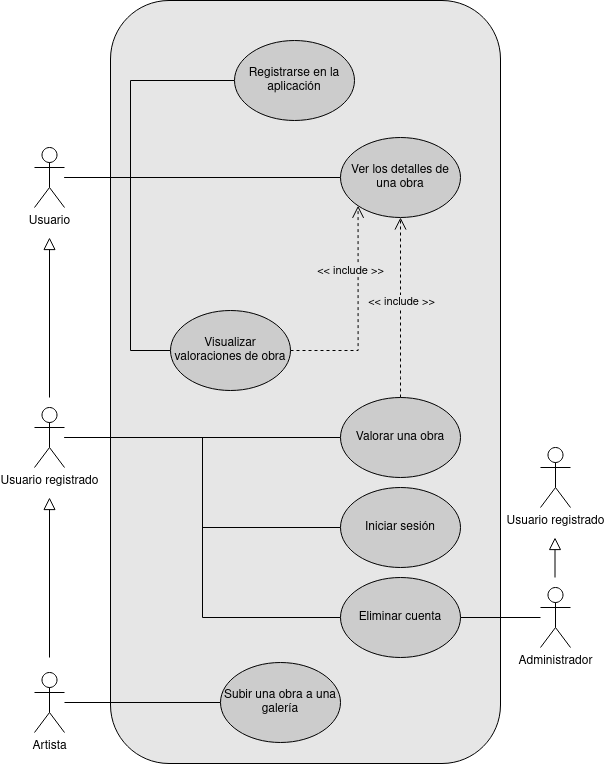
\includegraphics[width=\textwidth]{diagramas/casos_de_uso.png}
    \caption{Diagrama de casos de uso}
    \label{fig:casos_de_uso}
\end{figure}

\begin{figure}[H]
    \centering
    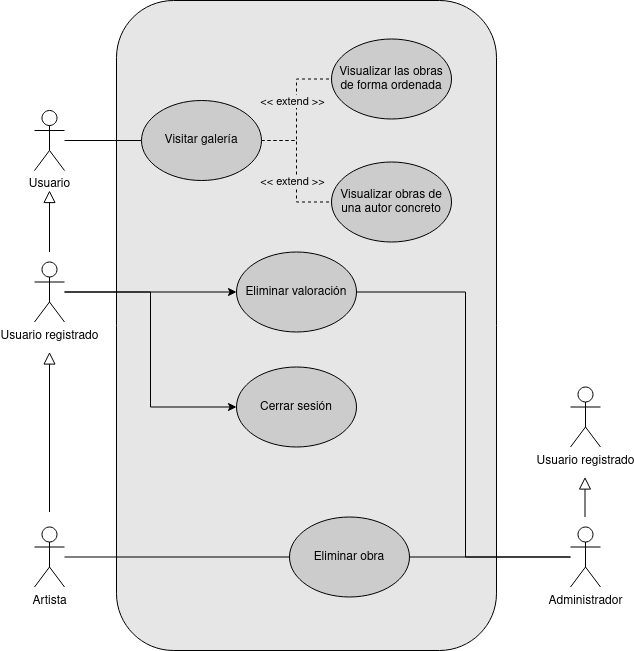
\includegraphics[width=\textwidth]{diagramas/casos_de_uso_2.png}
    \caption{Diagrama de casos de uso (continuación)}
    \label{fig:casos_de_uso_continuacion}
\end{figure}

\newpage
\section{Diagramas de secuencia}
A continuación se van a mostrar los diagramas de secuencia, también realizados
con la herramienta \textit{diagrams.net} \cite{diagramsnet}:

\begin{figure}[h]
    \centering
    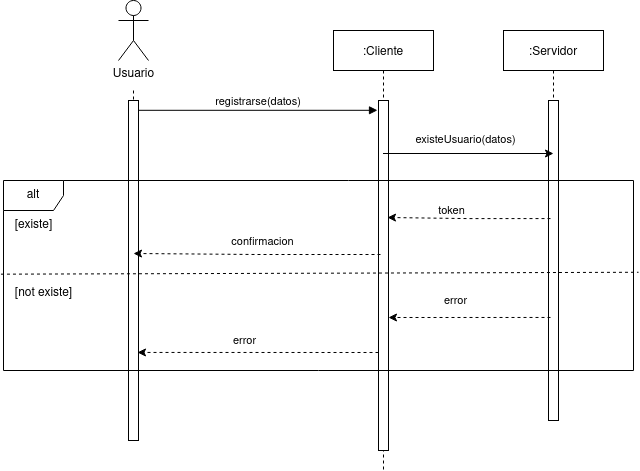
\includegraphics[width=\textwidth]{diagramas/secuencia_registrarse.png}
    \caption{Diagrama de secuencia de registrarse}
    \label{fig:registrarse}
\end{figure}

\begin{figure}[h]
    \centering
    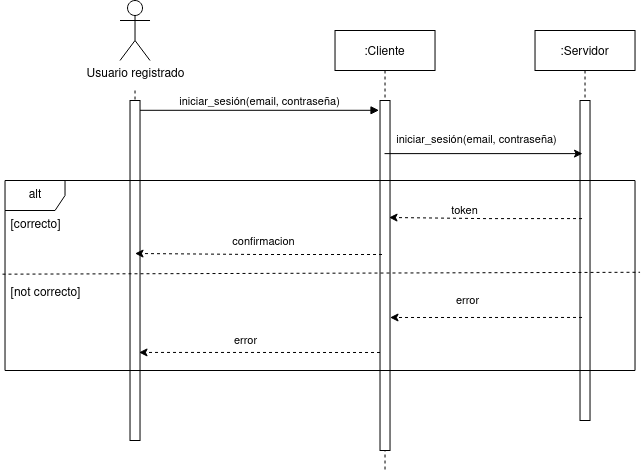
\includegraphics[width=\textwidth]{diagramas/secuencia_iniciar_sesion.png}
    \caption{Diagrama de secuencia de iniciar sesión}
    \label{fig:iniciar_sesion}
\end{figure}

\begin{figure}[h]
    \centering
    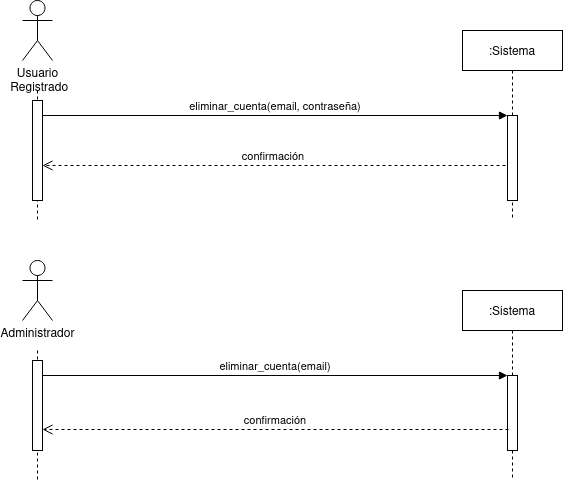
\includegraphics[width=\textwidth]{diagramas/secuencia_eliminar_cuenta.png}
    \caption{Diagrama de secuencia de eliminar cuenta}
    \label{fig:eliminar_cuenta}
\end{figure}

\begin{figure}[h]
    \centering
    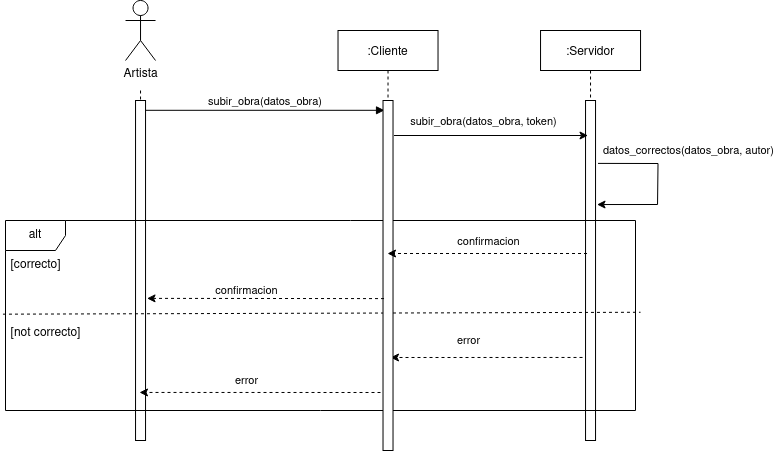
\includegraphics[width=\textwidth]{diagramas/secuencia_subir_obra.png}
    \caption{Diagrama de secuencia de subir obra}
    \label{fig:subir_obra}
\end{figure}

\begin{figure}[h]
    \centering
    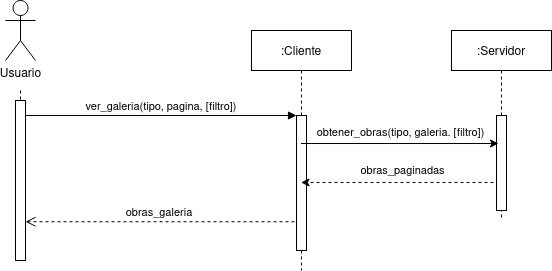
\includegraphics[width=\textwidth]{diagramas/secuencia_mostrar_galeria.png}
    \caption{Diagrama de secuencia de mostrar galería}
    \label{fig:mostrar_galeria}
\end{figure}

\begin{figure}[h]
    \centering
    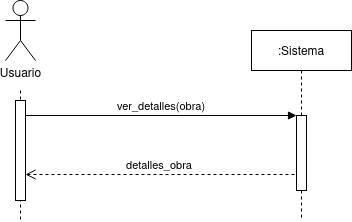
\includegraphics[width=\textwidth]{diagramas/secuencia_mostrar_detalles_obra.png}
    \caption{Diagrama de secuencia de mostrar detalles de obra}
    \label{fig:mostrar_detalles_obra}
\end{figure}

\begin{figure}[h]
    \centering
    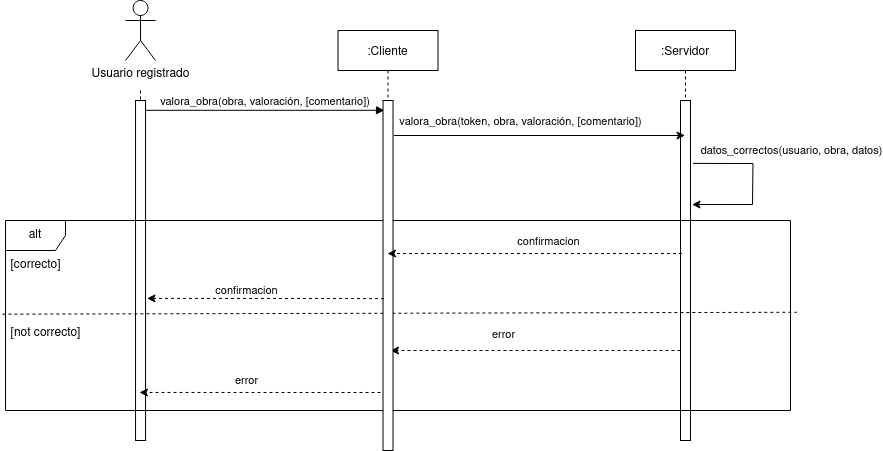
\includegraphics[width=\textwidth]{diagramas/secuencia_valorar_obra.png}
    \caption{Diagrama de secuencia de valorar obra}
    \label{fig:valorar_obra}
\end{figure}
